\section{Esercizio 12}
\textit{\textbf{Descrizione:} crivere una function Matlab che, data in ingresso la matrice \textbf{QR} creata dalla function del precedente esercizio, ed il termine noto del sistema lineare \textbf{Ax = b}, ne calcoli la soluzione nel senso dei minimi quadrati: function \textbf{x = qrsolve(QR,b)}. Curare particolarmente la scrittura e l'efficienza della function.}\newline
\noindent \textit{\textbf{Svolgimento:}}\newline
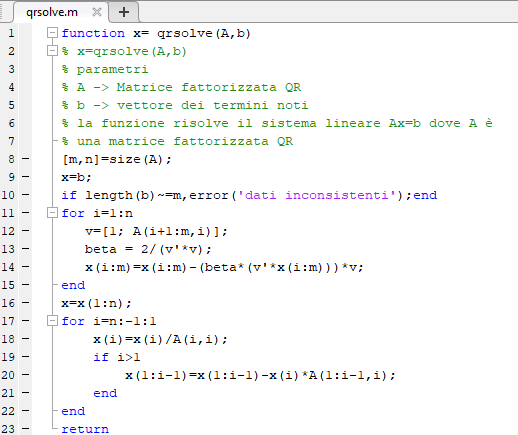
\includegraphics[width=1.3\linewidth]{img/qrsolve.png}\newpage